%\newpage
\section{Tecnologie}
	L'obiettivo di questo paragrafo è quello di descrivere in modo generale come il prodotto andrà ad interfacciarsi con le tecnologie che mandano e ricevono le notifiche che passano attraverso \progetto.\\
	Per ciascuna di queste tecnologie con cui l'\gloss{applicativo} andrà ad interfacciarsi è previsto un \gloss{microservizio}, il quale avrà come scopo quello di fare da tramite tra lo strumento che genera il messaggio e quello che lo riceve.\\
	Questo pattern si chiama Publisher / Subscriber e utilizza uno strumento intermedio detto Broker per lo smistamento dei messaggi e la gestione dei flussi.

	\begin{figure}[H]
		\centering
		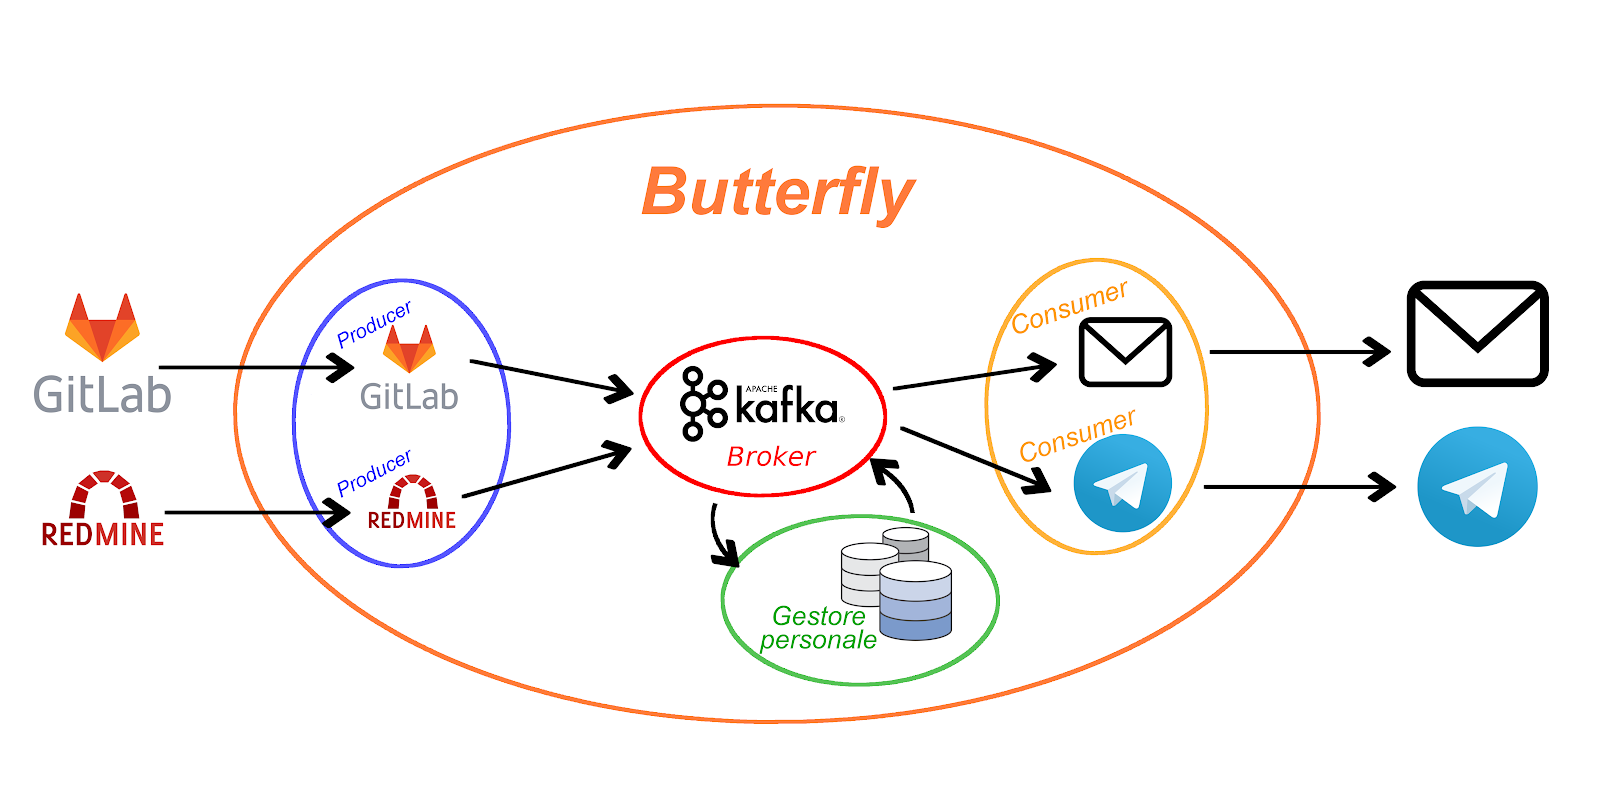
\includegraphics[width=\textwidth]{img/butterfly.png}\\
		\caption{Visione generale del sistema \progetto}
		\label{fig:butterfly}
	\end{figure}
	L'immagine precedente rappresenta una suddivisione del sistema in quattro sezioni principali:
	\begin{itemize}
		\item \progetto (arancione)
		\item \gloss{Producers} (azzurro)
		\item Broker (rosso)
		\item Consumers (verde)
	\end{itemize}
	Questa scomposizione permette di analizzare più approfonditamente il prodotto per la stesura dei casi d'uso, utilizzando come attori non solo le tecnologie esterne a Butterfly (GitLab, Redmine, Telegram ed e-mail) ma anche i microservizi interni come i Producer / Consumer associati e il Broker.
	
	\subsection{Producers}
	
		Per ciascuno degli strumenti che inviano messaggi verso il sistema è necessario creare un microservizio di tipo producer che li riceva ed li elabori inoltrandoli successivamente verso il Broker.
		Le tecnologie dalle quali vengono ricevuti i messaggi sono elencate di seguito in ordine di priorità in base a quanto richiesto dal committente.

		\subsubsection{Redmine}
		Ciascuna istanza di Redmine permette l'utilizzo delle proprie API\footnote{Riferirsi alla voce "API Rest di Redmine" alla sezione \S\ref{sec:RiferimentiInformativi}} con le quali è possibile interfacciarsi e ricevere risposte nel formato scelto.
		Queste vengono prese dal server tramite un microservizio che ne fa la richiesta ad intervalli prestabiliti, aggiornando in base a quello che riceve i dati presenti sul gestore personale e inoltrando le notifiche ai customer interessati.
		
		\subsubsection{GitLab}
		Ciascuna istanza di GitLab, online o in un server locale interno dell'azienda, mette a disposizione la configurazione di webhooks\footnote{Riferirsi alla voce "Weebhooks di GitLab" alla sezione \S\ref{sec:RiferimentiInformativi}} che, alla modifica della \gloss{repository}, manda un messaggio con le informazioni dei cambiamenti, inseriti nella repository, a un microservizio capace di aggiornare i dati presenti nel gestore personale e, come prima, inoltrare le notifiche ai customer interessati.
		
%		\subsubsection{SonarQube}
%		Come GitLab, anche SonarQube prevede l'utilizzo di webhooks\footnote{\url{https://docs.sonarqube.org/latest/project-administration/webhooks/}} che dopo ciascuna build comunica il risultato e le informazioni relative ad essa ad un microservizio capace di aggiornare i dati presenti nel gestore personale e, anche in questo caso, inoltrare le notifiche ai customer interessati.
		
	\subsection{Broker}
	
		Il ruolo del Broker è quello smistare i messaggi in base ai Topic con cui questi sono contrassegnati verso i vari microservizi con cui l'utente ha deciso che gli venga inoltrata la notifica.
		L'azienda consiglia di utilizzare come broker per i messaggi Apache Kafka.
	
		\subsubsection{Apache Kafka}
		\gloss{Apache Kafka} è un software \gloss{open source} che permette la lettura e la scrittura di messaggi su stream di dati.
		Questi messaggi arrivano dai microservizi producer che ricevono le notifiche di applicazioni di terze parti e mandandole verso il Broker. Questo le elabora analizzandone il contenuto e contrassegnandole con Topic che verranno utilizzati per l'inoltro ai Consumer e successivamente agli utenti finali, i quali possono abbonarsi a più Topic e gestendo le proprie preferenze.
		
	
	\subsection{Consumers}
		Come per gli strumenti precedentemente elencati, anche per quelli su cui il messaggio andrà ad essere inoltrato, è necessaria la creazione di un microservizio in grado di fare da tramite tra Broker e client dello strumento.
		Le tecnologie alle quali vengono inoltrati i messaggi sono elencate di seguito in ordine di priorità in base a quanto richiesto dal committente.
			
		\subsubsection{Telegram}
		Telegram permette l'interazione in maniera automatica con gli utenti tramite \gloss{bot} che possono essere configurati per mandare messaggi ricevuti da strumenti di terze parti.
		Il Broker manda i messaggi ad un microservizio che si occupa della trasmissione effettiva al bot di Telegram.
		%https://core.telegram.org/bots
		
		\subsubsection{E-mail}
		Per inoltrare le e-mail agli utenti finali è necessario un microservizio che sfrutta un server di posta in modo tale da poter ricevere i messaggi dal Broker e poi mandarli all'indirizzo specificato.
		%https://realpython.com/python-send-email/
		
%		\subsubsection{Slack}
%		È possibile utilizzare le API di Slack per poter mandare push notifications ai canali o alle persone interessate specificando il nome del canale (o lo username della persona), testo del messaggio, e lo username che verrà mostrato per il mittente.
%		%https://www.confluent.io/blog/real-time-syslog-processing-with-apache-kafka-and-ksql-part-2-event-driven-alerting-with-slack/
	
	\subsection{Gestore personale}
	Il gestore personale è quel componente che permette agli utenti di impostare le proprie preferenze per il canale di inoltro dei messaggi ed i Topic a cui ci si iscrive, interfacciandosi dunque con l'intero sistema.
	È previsto come un'applicazione web installata in un server interno all'azienda accessibile dai dipendenti interessati, i quali potranno quindi modificare, perciò con la possibilità di aggiungere e rimuovere, impostazioni come Topic a cui si è iscritti e modalità di ricezione dei messaggi.
	
	\subsection{Container Software}
	
		Un container software simula questo ambiente virtuale dove è possibile testare e mantenere le proprie applicazioni, permettendo di aumentare l'efficienza riducendone i costi e simulando l'esecuzione di sistema operativo su una macchina con risorse condivise.
		
		\subsection{Differenza tra container e macchina virtuale}
		A differenza delle macchine virtuali, dove lo stato dell'ambiente viene salvato su disco occupando memoria, i container si adattano in maniera più performante all'applicativo richiesto, in quanto il loro scopo è quello di massimizzare la quantità delle applicazioni in esecuzione riducendo al minimo il numero delle macchine per eseguirla.
		Sono quindi più leggeri, occupando meno memoria su disco e impiegando meno risorse. Purtroppo al termine della loro esecuzione non viene salvato lo stato, a meno che non sia esplicitamente richiesto.
		
		\subsubsection{Docker e Dockerfile}
		L'azienda consiglia di utilizzare Docker per la semplicità e perché si adatta all'architettura a microservizi.
		La configurazione avverrà tramite un dockerfile in cui verranno specificate informazioni come sistema operativo, script di avvio, numero di istanze ed altri parametri specifici.
